\pdfminorversion=4
\documentclass[aspectratio=169]{beamer}

\mode<presentation>
{
  \usetheme{default}
  \usecolortheme{default}
  \usefonttheme{default}
  \setbeamertemplate{navigation symbols}{}
  \setbeamertemplate{caption}[numbered]
  \setbeamertemplate{footline}[frame number]  % or "page number"
  \setbeamercolor{frametitle}{fg=white}
  \setbeamercolor{footline}{fg=black}
} 

\usepackage[english]{babel}
\usepackage[utf8x]{inputenc}
\usepackage{tikz}
\usepackage{courier}
\usepackage{array}
\usepackage{bold-extra}
\usepackage{minted}
\usepackage[thicklines]{cancel}
\usepackage{fancyvrb}

\xdefinecolor{dianablue}{rgb}{0.18,0.24,0.31}
\xdefinecolor{darkblue}{rgb}{0.1,0.1,0.7}
\xdefinecolor{darkgreen}{rgb}{0,0.5,0}
\xdefinecolor{darkgrey}{rgb}{0.35,0.35,0.35}
\xdefinecolor{darkorange}{rgb}{0.8,0.5,0}
\xdefinecolor{darkred}{rgb}{0.7,0,0}
\definecolor{darkgreen}{rgb}{0,0.6,0}
\definecolor{mauve}{rgb}{0.58,0,0.82}

\title[2022-05-23-analysis-ux-python-hep]{Pythonic HEP ecosystem update}
\author{Jim Pivarski}
\institute{Princeton University -- IRIS-HEP}
\date{May 23, 2022}

\usetikzlibrary{shapes.callouts}

\begin{document}

\logo{\pgfputat{\pgfxy(0.11, 7.4)}{\pgfbox[right,base]{\tikz{\filldraw[fill=dianablue, draw=none] (0 cm, 0 cm) rectangle (50 cm, 1 cm);}\mbox{\hspace{-8 cm}\includegraphics[height=1 cm]{princeton-logo-long.png}\hspace{0.1 cm}\raisebox{0.1 cm}{\includegraphics[height=0.8 cm]{iris-hep-logo-long.png}}\hspace{0.1 cm}}}}}

\begin{frame}
  \titlepage
\end{frame}

\logo{\pgfputat{\pgfxy(0.11, 7.4)}{\pgfbox[right,base]{\tikz{\filldraw[fill=dianablue, draw=none] (0 cm, 0 cm) rectangle (50 cm, 1 cm);}\mbox{\hspace{-8 cm}\includegraphics[height=1 cm]{princeton-logo.png}\hspace{0.1 cm}\raisebox{0.1 cm}{\includegraphics[height=0.8 cm]{iris-hep-logo.png}}\hspace{0.1 cm}}}}}

% Uncomment these lines for an automatically generated outline.
%\begin{frame}{Outline}
%  \tableofcontents
%\end{frame}

% START START START START START START START START START START START START START

\begin{frame}{From the first Analysis Ecosystem Workshop report (4 Aug 2017)}
\vspace{0.5 cm}
\begin{columns}
\column{1.1\linewidth}
\includegraphics[width=\linewidth]{PLOTS/ecosystem-2017-python-first-class-2.png}
\end{columns}
\end{frame}

\begin{frame}{Back then, Python was just beginning to take over data analytics}
\vspace{0.25 cm}
\textcolor{darkblue}{Source: Google Analytics, worldwide search traffic.}

\vspace{-0.3 cm}
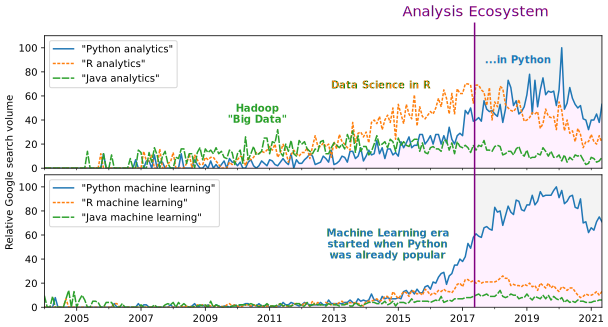
\includegraphics[width=\linewidth]{PLOTS/analytics-by-language.pdf}
\end{frame}

\begin{frame}{Though it had been slowly growing in HEP for years}
\vspace{0.25 cm}
\textcolor{darkblue}{Source: Title and abstract matches in CHEP proceedings.}

\vspace{-0.3 cm}
\mbox{ } \hfill 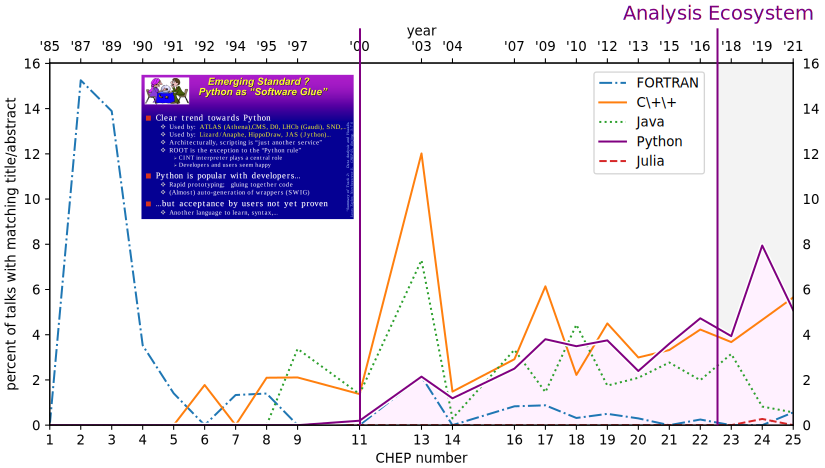
\includegraphics[width=0.95\linewidth]{PLOTS/chep-papers-language-2.pdf} \hfill \mbox{ }
\end{frame}

\begin{frame}{But the use of Scientific Python (NumPy, etc.) was new to HEP}
\vspace{0.25 cm}
\textcolor{darkblue}{Source: ``\mintinline{python}{import XYZ}'' matches in GitHub repos for users who fork CMSSW.}

\includegraphics[width=\linewidth]{PLOTS/gihub-package-fullstudy-for-review.pdf}
\end{frame}

\begin{frame}{Scikit-HEP had not yet taken off}
\vspace{0.25 cm}
\textcolor{darkblue}{Source: ``\mintinline{bash}{pip install XYZ}'' download rate for MacOS/Windows (no batch jobs).}

\vspace{0.1 cm}
\only<1>{\includegraphics[width=\linewidth]{PLOTS/pip-macwin-scikithep-log-for-report-0.pdf}}\only<2>{\includegraphics[width=\linewidth]{PLOTS/pip-macwin-scikithep-log-for-report.pdf}}
\end{frame}

\begin{frame}{We are now a two-language community}
\vspace{0.25 cm}
\textcolor{darkblue}{Source: PyHEP 2020 workshop survey.}

\vspace{-0.3 cm}
\begin{columns}
\column{1.15\linewidth}
\includegraphics[width=\linewidth]{PLOTS/pyhep2020-survey-5.pdf}
\end{columns}
\end{frame}


\begin{frame}{}

\end{frame}

\begin{frame}{uproot-browser}
\vspace{0.35 cm}
\begin{center}
\only<1>{\includegraphics[width=0.9\linewidth]{PLOTS/uproot-browser-tui-frames/00.png}}\only<2>{\includegraphics[width=0.9\linewidth]{PLOTS/uproot-browser-tui-frames/01.png}}\only<3>{\includegraphics[width=0.9\linewidth]{PLOTS/uproot-browser-tui-frames/02.png}}\only<4>{\includegraphics[width=0.9\linewidth]{PLOTS/uproot-browser-tui-frames/03.png}}\only<5>{\includegraphics[width=0.9\linewidth]{PLOTS/uproot-browser-tui-frames/04.png}}\only<6>{\includegraphics[width=0.9\linewidth]{PLOTS/uproot-browser-tui-frames/05.png}}\only<7>{\includegraphics[width=0.9\linewidth]{PLOTS/uproot-browser-tui-frames/06.png}}\only<8>{\includegraphics[width=0.9\linewidth]{PLOTS/uproot-browser-tui-frames/07.png}}\only<9>{\includegraphics[width=0.9\linewidth]{PLOTS/uproot-browser-tui-frames/08.png}}\only<10>{\includegraphics[width=0.9\linewidth]{PLOTS/uproot-browser-tui-frames/09.png}}\only<11>{\includegraphics[width=0.9\linewidth]{PLOTS/uproot-browser-tui-frames/10.png}}\only<12>{\includegraphics[width=0.9\linewidth]{PLOTS/uproot-browser-tui-frames/11.png}}\only<13>{\includegraphics[width=0.9\linewidth]{PLOTS/uproot-browser-tui-frames/12.png}}\only<14>{\includegraphics[width=0.9\linewidth]{PLOTS/uproot-browser-tui-frames/13.png}}\only<15>{\includegraphics[width=0.9\linewidth]{PLOTS/uproot-browser-tui-frames/14.png}}\only<16>{\includegraphics[width=0.9\linewidth]{PLOTS/uproot-browser-tui-frames/15.png}}\only<17>{\includegraphics[width=0.9\linewidth]{PLOTS/uproot-browser-tui-frames/16.png}}\only<18>{\includegraphics[width=0.9\linewidth]{PLOTS/uproot-browser-tui-frames/17.png}}\only<19>{\includegraphics[width=0.9\linewidth]{PLOTS/uproot-browser-tui-frames/18.png}}\only<20>{\includegraphics[width=0.9\linewidth]{PLOTS/uproot-browser-tui-frames/19.png}}\only<21>{\includegraphics[width=0.9\linewidth]{PLOTS/uproot-browser-tui-frames/20.png}}\only<22>{\includegraphics[width=0.9\linewidth]{PLOTS/uproot-browser-tui-frames/21.png}}\only<23>{\includegraphics[width=0.9\linewidth]{PLOTS/uproot-browser-tui-frames/22.png}}\only<24>{\includegraphics[width=0.9\linewidth]{PLOTS/uproot-browser-tui-frames/23.png}}\only<25>{\includegraphics[width=0.9\linewidth]{PLOTS/uproot-browser-tui-frames/24.png}}\only<26>{\includegraphics[width=0.9\linewidth]{PLOTS/uproot-browser-tui-frames/25.png}}\only<27>{\includegraphics[width=0.9\linewidth]{PLOTS/uproot-browser-tui-frames/26.png}}\only<28>{\includegraphics[width=0.9\linewidth]{PLOTS/uproot-browser-tui-frames/27.png}}\only<29>{\includegraphics[width=0.9\linewidth]{PLOTS/uproot-browser-tui-frames/28.png}}\only<30>{\includegraphics[width=0.9\linewidth]{PLOTS/uproot-browser-tui-frames/29.png}}\only<31>{\includegraphics[width=0.9\linewidth]{PLOTS/uproot-browser-tui-frames/30.png}}\only<32>{\includegraphics[width=0.9\linewidth]{PLOTS/uproot-browser-tui-frames/31.png}}
\end{center}
\end{frame}


\begin{frame}{}

\end{frame}


\end{document}
